\documentclass[poly]{valbonne}

% Les macros etc
%%%%%%%%%%%%%%%%%%%% COMMANDES DES ANIMATHEURS



\begin{document}


% Intro
\newgeometry{left=19mm,right=19mm,top=17mm,bottom=11mm}

\begin{center}\LARGE{\textsc{STAGE OLYMPIQUE DE VALBONNE 2021}}
\vrule depth 0pt height 0.4pt width 16cm\end{center}


%\medskip

%\begin{center}
%
\includegraphics[scale=0.15]{1-Intro/logos/animath.jpg}
%\end{center}

%\vspace*{0.5}

%\medskip
\vspace{2cm}


\begin{center}

\includegraphics[height=12cm]{1-Intro/logos/tous.jpg}
\end{center}

%\vspace{0.5cm}

%\vspace*{0.5cm}
%\begin{center}du 16 au 26 août 2021\end{center}


%% MODIFIER LA LISTE DES LOGOS...


\begin{figure*}[h!]
	
	\vspace{1cm}
	
	\centering
  \begin{minipage}[c]{4cm}
     \centering
	   
\includegraphics[width=5cm]{1-Intro/logos/animath.jpg}
   \end{minipage}
   
   \vspace{2cm}

   \begin{minipage}[c]{4cm}
   \centering
        \includegraphics[width=4cm]{1-Intro/logos/EN.jpg}
   \end{minipage} \hfill
   \begin{minipage}[c]{2cm}
   \centering
      
\includegraphics[width=1.5cm]{1-Intro/logos/cnrs.jpg}
   \end{minipage} \hfill \hskip 1cm
   \begin{minipage}[c]{2cm}
   \centering
      
\includegraphics[width=2cm]{1-Intro/logos/inria.png}
   \end{minipage}
   
   \bigskip

   \begin{minipage}[c]{2cm}
   \centering
   
\includegraphics[width=2cm]{1-Intro/logos/polytechnique.jpg}
   \end{minipage} \hskip 2cm \hfill
      \begin{minipage}[c]{2cm}
   \centering
        
\includegraphics[width=2cm]{1-Intro/logos/texas.jpg}
   \end{minipage} \hfill
   \begin{minipage}[c]{3cm}
   \centering
      
\includegraphics[width=3cm]{1-Intro/logos/fondation_blaise_pascal.jpg}
   \end{minipage} 
   
   \bigskip
   
   \begin{minipage}[c]{2cm}
   \centering
        
\includegraphics[width=2cm]{1-Intro/logos/cm.jpg}
   \end{minipage}  \hskip 2cm \hfill
   \begin{minipage}[c]{2cm}
   \centering
      
\includegraphics[width=2cm]{1-Intro/logos/casio.jpg}
   \end{minipage} \hfill \hskip 1cm
   	\begin{minipage}[c]{2cm}
   \centering
      
\includegraphics[width=2cm]{1-Intro/logos/fondation_societe_generale.jpg}
   \end{minipage} 
   
   
\end{figure*}

\restoregeometry

\pagestyle{empty}~

 \pagebreak



\clearpage

\vspace*{\stretch{1}}

\begin{flushright}

\textbf{\Large{Avant-propos}}

\bigskip

\emph{Le stage olympique de Valbonne 2021 a été organisé par l'association Animath.}

\bigskip

\emph{Son objet a été de rassembler 80 collégiennes, collégiens,\\
lycéennes et lycéens de la quatrième à la terminale, \\
de 12 à 17 ans, passionnés de mathématiques \\
sélectionnés parmi les près de 700 candidats à la Coupe Animath, \\
dont certains représenteront la France aux compétitions internationales : \\
Olympiades Internationales de Mathématiques (IMO), \\
Olympiades Balkaniques Junior de Mathématiques (JBMO), \\
Olympiades Européennes de Filles de Mathématiques (EGMO), \\
Romanian Masters of Mathematics (RMM), \\ 
Mediterranean Youth Mathematical Championship (MYMC), \\
Olympiade Francophone de Mathématiques (OFM).}

\bigskip

\emph{
Environ la moitié des stagiaires ont pu découvrir la beauté des mathématiques olympiques,\\
tandis que l'autre moitié, ayant déjà une petite expérience dans ce domaine,\\
a pu approfondir ses connaissances.\\
Toute l'équipe représentant la France pour les IMO de cette année était présente,\\
et a bénéficié d'une préparation particulière dans l'inédit groupe E...\\
}
 
\vspace{3cm}

\emph{Nous tenons à remercier le Centre International de Valbonne pour son excellent accueil.}
\end{flushright}

\vspace*{\stretch{1}}



\pagebreak

\mbox { }

\pagebreak




% Deroulement
\begin{center}
{\Huge\textbf{Déroulement du stage}}
\end{center}
\vspace{2mm}

Pour la 5ième fois, le Centre International de Valbonne (CIV) nous a accueilli du lundi 16 août vers 15h au jeudi 26 août vers 8h, avec un effectif final de 79 stagiaires et 28 animatheurs. 

%TODO : Mathieu/Arthur doit donner les stats
Parmi les presque XX candidats à la Coupe Animath, 700 ont franchi le cap du premier tour. Sur la base des résultats du second tour, nous devions accueillir 79 stagiaires, dont environ 31 de fin de première, 18 de seconde, 19 de troisième et 12 de quatrième. En prévision des EGMO, Olympiades Européennes Féminines de Mathématiques, et de la JBMO, Olympiades Balkaniques Junior de Mathématiques, des bonifications ont été ajoutées pour favoriser les filles et les plus jeunes.




Le stage était structuré comme ceux des années précédentes : deux périodes de quatre jours (18 - 21 août et 22 - 26 août), trois de cours / exercices, un entraînement %(test) 
de type olympique le matin du quatrième jour (de 9h à 12h, ou, pour le groupe D, de 8h à 12h) et une après-midi récréative. Les élèves étaient répartis en 4 groupes A, B, C, et D en fonction de leur expérience en mathématiques olympiques.
Le programme est construit suivant ce qui est demandé lors des compétitions internationales : Arithmétique, Algèbre, Combinatoire et Géométrie.



En plus des cours étaient prévues, le soir, des conférences à vocation culturelle, permettant de découvrir de nouveaux pans des mathématiques. Merci à Pooran Memari pour son exposé sur les triangulations et leur utilisation dans la vie courante ; Colin Davalo pour sa présentation des jeux combinatoires (et avoir appris aux élèves à gagner à tous les coups au jeu de Nim !) ; Phong Nguyen pour son colloque sur l'utilisation de la théorie des nombres dans la vie courante et à Victor Vermès pour sa (très actuelle) conférence sur la propagation d'une épidémie.



L'après-midi suivant le premier entraînement fut organisée un grand jeu par une petite équipe chapeautée par X. % METTRE UN PETIT COMMENTAIRE, et rajouter ce qui s'est passé lors du second entraînement.


Il est possible de retrouver les comptes rendus du stage au jour le jour sur le site de la POFM : \url{https://maths-olympiques.fr/?p=7488}

\vfill
\pagebreak



\newpage
\thispagestyle{empty}
\mbox{ }
%\newpage

% Les trombis
\pagestyle{plain}
\footnotesize
\newcommand{\ssspas}{2.9cm}
\renewcommand{\headrulewidth}{0pt}
\setlength{\tabcolsep}{6pt}
\addtolength{\voffset}{-1.2cm}
\addtolength{\textheight}{2.4cm}
%
%% trombi profs
%\graphicspath{{PTR/001-Intro/trombi-profs/}}
%\input{PTR/trombi-profs}
%% trombi eleves
%\graphicspath{{PTR/01-Intro/trombi-eleves/}}
%\titre{Les élèves}

%\vfill

\vspace{2mm}
\begin{center}
\begin{tabular}{cccc}

\includegraphics[angle=270,origin=c, width=27mm]{eleves/Averous Paul.JPG} &

\includegraphics[angle=270,origin=c, width=27mm]{eleves/Baradel Pauline.JPG} &

\includegraphics[angle=270,origin=c, width=27mm]{vide.JPG} &

\includegraphics[angle=270,origin=c, width=27mm]{eleves/Bidallier Serge.JPG} \\
Paul Avérous & Pauline Baradel & Clément Beau & Serge Bidallier \\ \\ \\


\includegraphics[angle=270,origin=c, width=27mm]{eleves/Boitier Kristen.JPG} &

\includegraphics[angle=270,origin=c, width=27mm]{eleves/Bouton Anatole.JPG} &
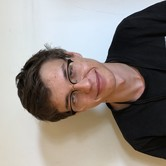
\includegraphics[angle=270,origin=c, width=27mm]{eleves/Causse Gaspard.JPG} &
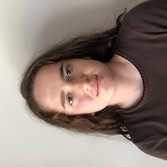
\includegraphics[angle=270,origin=c, width=27mm]{eleves/Cerf Nelly.JPG} \\
Kristen Boitier & Anatole Bouton & Gaspard Causse & Nelly Cerf \\ \\ \\


\includegraphics[angle=270,origin=c, width=27mm]{eleves/Chabot Sophia.JPG} &
\includegraphics[angle=270,origin=c, width=27mm]{eleves/Choné Axel.JPG} &
\includegraphics[angle=270,origin=c, width=27mm]{eleves/Choné Lancelot.JPG} &

\includegraphics[angle=270,origin=c, width=27mm]{eleves/Cloup Lucile.JPG} \\
Sophia Chabot & Axel Choné & Lancelot Choné & Lucile Cloup \\ \\ \\


\includegraphics[angle=270,origin=c, width=27mm]{eleves/Cormier Faustas.JPG} &

\includegraphics[angle=270,origin=c, width=27mm]{eleves/Corot Eva.JPG} &

\includegraphics[angle=270,origin=c, width=27mm]{eleves/Dai Charles.JPG} &

\includegraphics[angle=270,origin=c, width=27mm]{eleves/Darmendrail Baudouin.JPG} \\
Faustas Cormier & Eva Corot & Charles Dai & Baudouin \\
 & & & Darmendrail \\ \\ \\

\includegraphics[angle=270,origin=c, width=27mm]{eleves/Dautzenberg Gaëtan.JPG} &

\includegraphics[angle=270,origin=c, width=27mm]{eleves/De Belloy Madeleine.JPG} &
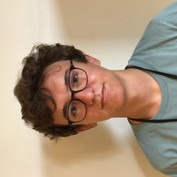
\includegraphics[angle=270,origin=c, width=27mm]{eleves/De Larouziere Jean.JPG} &

\includegraphics[angle=270,origin=c, width=27mm]{eleves/Delabre Gaspard.JPG} \\
Gaëtan & Madeleine & Jean & Gaspard Delabre \\ Dautzenberg & De Belloy & De Larouzière & \\ \\ \\

\end{tabular}
\end{center}

\vfill
\pagebreak

\begin{center}
\begin{tabular}{cccc}

\includegraphics[angle=270,origin=c, width=27mm]{eleves/Deloye Claire.JPG} &
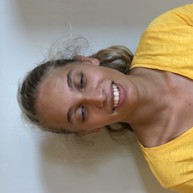
\includegraphics[angle=0,origin=c, width=27mm]{eleves/Di Mascolo Capucine.JPG} &
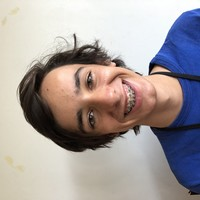
\includegraphics[angle=270,origin=c, width=27mm]{eleves/Dognon Antoine.JPG} &
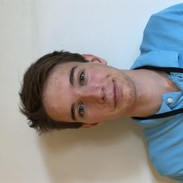
\includegraphics[angle=270,origin=c, width=27mm]{eleves/Duchemin Aimeric.JPG} \\
Claire Deloye & Capucine & Antoine Dognon & Aimeric \\ & Di Mascolo & & Duchemin \\ \\ \\


\includegraphics[angle=270,origin=c, width=27mm]{eleves/Dürrüoglu Pierre Akin.JPG} &
\includegraphics[angle=270,origin=c, width=27mm]{eleves/Etilé Mano.JPG} &
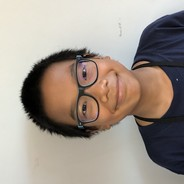
\includegraphics[angle=270,origin=c, width=27mm]{eleves/Faucheu Hadrien.JPG} &

\includegraphics[angle=270,origin=c, width=27mm]{eleves/Faucheu Hannah.JPG} \\
Pierre-Akin & Mano Étilé & Hadrien & Hannah Faucheu \\ Dürrüoglu & & Faucheu &\\ \\ \\


\includegraphics[angle=270,origin=c, width=27mm]{eleves/Fonteniaud Claire.JPG} &
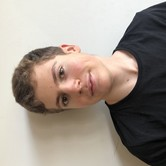
\includegraphics[angle=270,origin=c, width=27mm]{eleves/Girel Nicolas.JPG} &
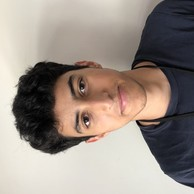
\includegraphics[angle=270,origin=c, width=27mm]{eleves/Hamimed Zinedine.JPG} &

\includegraphics[angle=270,origin=c, width=27mm]{eleves/Henrotte Guillaume.JPG} \\
Claire & Nicolas Girel & Zinedine & Guillaume \\ Fonteniaud & & Hamimed & Henrotte \\ \\ \\

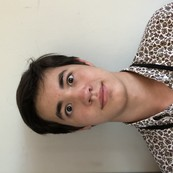
\includegraphics[angle=270,origin=c, width=27mm]{eleves/Henry Olivier.JPG} &
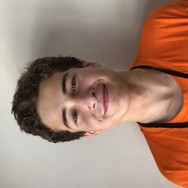
\includegraphics[angle=270,origin=c, width=27mm]{eleves/Hovasse Axel.JPG} &
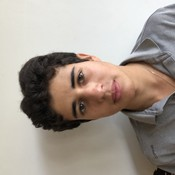
\includegraphics[angle=270,origin=c, width=27mm]{eleves/Hovasse Henri.JPG} &
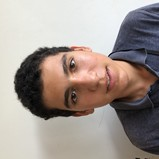
\includegraphics[angle=270,origin=c, width=27mm]{eleves/Ismaaili Erny Noam.JPG} \\
Olivier Henry & Axel Hovasse & Henri Hovasse & Noam Erny-\\ & & & Ismaaili \\ \\ \\

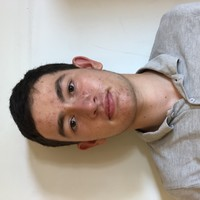
\includegraphics[angle=270,origin=c, width=27mm]{eleves/Israël Itaï.JPG} &
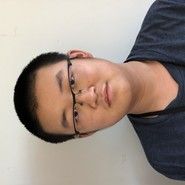
\includegraphics[angle=270,origin=c, width=27mm]{eleves/Jiang Tianrui.JPG} &
\includegraphics[angle=270,origin=c, width=27mm]{eleves/Jouani Loqman.JPG} &
\includegraphics[angle=270,origin=c, width=27mm]{eleves/Kouhkan Maryam.JPG} \\
Itaï Israël & Tianrui Jiang & Loqman Jouani & Maryam \\ & & & Kouhkan \\ \\ \\

\includegraphics[angle=270,origin=c, width=27mm]{eleves/Landau Nathan.JPG} &
\includegraphics[angle=270,origin=c, width=27mm]{eleves/Landau Salomé.JPG} &
\includegraphics[angle=270,origin=c, width=27mm]{eleves/Langé Quentin.JPG} &
\includegraphics[angle=270,origin=c, width=27mm]{eleves/Laurent-Levinson Paul.JPG} \\
Nathan Landau & Salomé Landau & Quentin Langé & Paul Laurent- \\ & & & Levinson\\ \\ \\

\end{tabular}
\end{center}
	
\vfill
\pagebreak

\begin{center}
\begin{tabular}{cccc}
\includegraphics[angle=270,origin=c, width=27mm]{eleves/Lbath Mounir.JPG} &
\includegraphics[angle=0,origin=c, width=27mm]{eleves/Le Berre Amédée.JPG} &
\includegraphics[angle=270,origin=c, width=27mm]{eleves/Legros Ronan.JPG} &
\includegraphics[angle=270,origin=c, width=27mm]{eleves/LescœurCorentin.JPG} \\
Mounir Lbath & Amédée Le Berre & Ronan Legros & Corentin \\ & & & Lescoeur \\ \\ \\

\includegraphics[angle=270,origin=c, width=27mm]{eleves/Lhssani Emma.JPG} &
\includegraphics[angle=270,origin=c, width=27mm]{eleves/Marcus Nicolas.JPG} &
\includegraphics[angle=270,origin=c, width=27mm]{eleves/Maris David.JPG} &
\includegraphics[angle=270,origin=c, width=27mm]{eleves/Milot Hadriel.JPG} \\
Emma Lhssani & Nicolas Marcus & Davis Maris & Hadriel Milot \\ \\ \\

\includegraphics[angle=270,origin=c, width=27mm]{eleves/Mingo Sol.JPG} &
\includegraphics[angle=270,origin=c, width=27mm]{eleves/Mischler Stanislas.JPG} &
\includegraphics[angle=270,origin=c, width=27mm]{eleves/Muñoz Mateo.JPG} &
\includegraphics[angle=270,origin=c, width=27mm]{eleves/Nistor Lucas.JPG} \\
Sol Mingo & Stanislas & Mateo Muñoz & Lucas Nistor \\ & Mischler & & \\ \\ \\

\includegraphics[angle=270,origin=c, width=27mm]{eleves/Pajaniradja Stéphane.JPG} &
\includegraphics[angle=270,origin=c, width=27mm]{eleves/Paun Alexandre.JPG} &
\includegraphics[angle=270,origin=c, width=27mm]{eleves/Pawlowski Camille.JPG} &
\includegraphics[angle=270,origin=c, width=27mm]{eleves/Pesquet Gabriel.JPG} \\
Stéphane & Alexandre & Camille & Gabriel Pesquet \\ Pajaniradja & Paun & Pawlowski & \\ \\ \\

\includegraphics[angle=270,origin=c, width=27mm]{eleves/Piednoir Jeanne.JPG} &
\includegraphics[angle=270,origin=c, width=27mm]{eleves/Priol Kevin.JPG} &
\includegraphics[angle=270,origin=c, width=27mm]{eleves/Ramondou Auguste.JPG} &
\includegraphics[angle=270,origin=c, width=27mm]{eleves/Regnier Camille.JPG} \\
Jeanne Piednoir & Kevin Priol & Auguste & Camille Regnier \\ & & Ramondou & \\ \\ \\

\includegraphics[angle=270,origin=c, width=27mm]{eleves/Roser Aurélien.JPG} &
\includegraphics[angle=270,origin=c, width=27mm]{eleves/Ruggeri Paul.JPG} &
\includegraphics[angle=270,origin=c, width=27mm]{eleves/Schwerer Raphaël.JPG} &
\includegraphics[angle=270,origin=c, width=27mm]{eleves/Souami Nell.JPG} \\
Aurélien Roser & Paul Ruggeri & Raphaël & Nell Souami \\ & & Schwerer & \\ \\ \\

\end{tabular}
\end{center}

\vfill
\pagebreak

\begin{center}
\begin{tabular}{cccc}
 \includegraphics[angle=270,origin=c, width=27mm]{eleves/Tézé Arthur.JPG} &
\includegraphics[angle=270,origin=c, width=27mm]{eleves/Tézé Georges.JPG} &
\includegraphics[angle=0,origin=c, width=27mm]{eleves/Thirion Alain.JPG} &
\includegraphics[angle=270,origin=c, width=27mm]{eleves/Triquenaux Amélie.JPG} \\
Arthur Tézé & Georges Tézé & Alain Thirion & Amélie \\ & & & Triquenaux \\ \\ \\

\includegraphics[angle=270,origin=c, width=27mm]{eleves/Van Der Hœven Niels.JPG} &
\includegraphics[angle=270,origin=c, width=27mm]{eleves/Verhille Elie.JPG} &
\includegraphics[angle=270,origin=c, width=27mm]{eleves/Viegas Yann.JPG} &
\includegraphics[angle=270,origin=c, width=27mm]{eleves/Visconti César.JPG} \\
Niels Van der & Élie Verhille & Yann Viegas & César Visconti \\ Hœven & & & \\ \\ \\

\includegraphics[angle=270,origin=c, width=27mm]{eleves/Vogel Matthieu.JPG} &
\includegraphics[angle=270,origin=c, width=27mm]{eleves/Zablocki Victor.JPG} &
\includegraphics[angle=270,origin=c, width=27mm]{eleves/Zheng Elisa.JPG} &
\includegraphics[angle=270,origin=c, width=27mm]{vide.JPG} \\
Matthieu Vogel & Victor Zablocki & Élisa Zheng & \\ \\ \\

\end{tabular}
\end{center}

%% trombi profs
%\graphicspath{{PTR/01-Intro/Trombinoscope/}}
%\input{PTR/trombi-profs}
% trombi eleves
%\graphicspath{{PTR/01-Intro/Trombinoscope/}}
%\titre{Les élèves}

%\vfill

\vspace{2mm}
\begin{center}
\begin{tabular}{cccc}
\includegraphics[angle=270,origin=c, width=27mm]{eleves/Averous Paul.JPG} &
\includegraphics[angle=270,origin=c, width=27mm]{eleves/Baradel Pauline.JPG} &
\includegraphics[angle=270,origin=c, width=27mm]{vide.JPG} &
\includegraphics[angle=270,origin=c, width=27mm]{eleves/Bidallier Serge.JPG} \\
Paul Avérous & Pauline Baradel & Clément Beau & Serge Bidallier \\ \\ \\

\includegraphics[angle=270,origin=c, width=27mm]{eleves/Boitier Kristen.JPG} &
\includegraphics[angle=270,origin=c, width=27mm]{eleves/Bouton Anatole.JPG} &
\includegraphics[angle=270,origin=c, width=27mm]{eleves/Causse Gaspard.JPG} &
\includegraphics[angle=270,origin=c, width=27mm]{eleves/Cerf Nelly.JPG} \\
Kristen Boitier & Anatole Bouton & Gaspard Causse & Nelly Cerf \\ \\ \\

\includegraphics[angle=270,origin=c, width=27mm]{eleves/Chabot Sophia.JPG} &
\includegraphics[angle=270,origin=c, width=27mm]{eleves/Choné Axel.JPG} &
\includegraphics[angle=270,origin=c, width=27mm]{eleves/Choné Lancelot.JPG} &
\includegraphics[angle=270,origin=c, width=27mm]{eleves/Cloup Lucile.JPG} \\
Sophia Chabot & Axel Choné & Lancelot Choné & Lucile Cloup \\ \\ \\

\includegraphics[angle=270,origin=c, width=27mm]{eleves/Cormier Faustas.JPG} &
\includegraphics[angle=270,origin=c, width=27mm]{eleves/Corot Eva.JPG} &
\includegraphics[angle=270,origin=c, width=27mm]{eleves/Dai Charles.JPG} &
\includegraphics[angle=270,origin=c, width=27mm]{eleves/Darmendrail Baudouin.JPG} \\
Faustas Cormier & Eva Corot & Charles Dai & Baudouin \\
 & & & Darmendrail \\ \\ \\

\includegraphics[angle=270,origin=c, width=27mm]{eleves/Dautzenberg Gaëtan.JPG} &
\includegraphics[angle=270,origin=c, width=27mm]{eleves/De Belloy Madeleine.JPG} &
\includegraphics[angle=270,origin=c, width=27mm]{eleves/De Larouziere Jean.JPG} &
\includegraphics[angle=270,origin=c, width=27mm]{eleves/Delabre Gaspard.JPG} \\
Gaëtan & Madeleine & Jean & Gaspard Delabre \\ Dautzenberg & De Belloy & De Larouzière & \\ \\ \\

\end{tabular}
\end{center}

\vfill
\pagebreak

\begin{center}
\begin{tabular}{cccc}
\includegraphics[angle=270,origin=c, width=27mm]{eleves/Deloye Claire.JPG} &
\includegraphics[angle=0,origin=c, width=27mm]{eleves/Di Mascolo Capucine.JPG} &
\includegraphics[angle=270,origin=c, width=27mm]{eleves/Dognon Antoine.JPG} &
\includegraphics[angle=270,origin=c, width=27mm]{eleves/Duchemin Aimeric.JPG} \\
Claire Deloye & Capucine & Antoine Dognon & Aimeric \\ & Di Mascolo & & Duchemin \\ \\ \\

\includegraphics[angle=270,origin=c, width=27mm]{eleves/Dürrüoglu Pierre Akin.JPG} &
\includegraphics[angle=270,origin=c, width=27mm]{eleves/Etilé Mano.JPG} &
\includegraphics[angle=270,origin=c, width=27mm]{eleves/Faucheu Hadrien.JPG} &
\includegraphics[angle=270,origin=c, width=27mm]{eleves/Faucheu Hannah.JPG} \\
Pierre-Akin & Mano Étilé & Hadrien & Hannah Faucheu \\ Dürrüoglu & & Faucheu &\\ \\ \\

\includegraphics[angle=270,origin=c, width=27mm]{eleves/Fonteniaud Claire.JPG} &
\includegraphics[angle=270,origin=c, width=27mm]{eleves/Girel Nicolas.JPG} &
\includegraphics[angle=270,origin=c, width=27mm]{eleves/Hamimed Zinedine.JPG} &
\includegraphics[angle=270,origin=c, width=27mm]{eleves/Henrotte Guillaume.JPG} \\
Claire & Nicolas Girel & Zinedine & Guillaume \\ Fonteniaud & & Hamimed & Henrotte \\ \\ \\

\includegraphics[angle=270,origin=c, width=27mm]{eleves/Henry Olivier.JPG} &
\includegraphics[angle=270,origin=c, width=27mm]{eleves/Hovasse Axel.JPG} &
\includegraphics[angle=270,origin=c, width=27mm]{eleves/Hovasse Henri.JPG} &
\includegraphics[angle=270,origin=c, width=27mm]{eleves/Ismaaili Erny Noam.JPG} \\
Olivier Henry & Axel Hovasse & Henri Hovasse & Noam Erny-\\ & & & Ismaaili \\ \\ \\

\includegraphics[angle=270,origin=c, width=27mm]{eleves/Israël Itaï.JPG} &
\includegraphics[angle=270,origin=c, width=27mm]{eleves/Jiang Tianrui.JPG} &
\includegraphics[angle=270,origin=c, width=27mm]{eleves/Jouani Loqman.JPG} &
\includegraphics[angle=270,origin=c, width=27mm]{eleves/Kouhkan Maryam.JPG} \\
Itaï Israël & Tianrui Jiang & Loqman Jouani & Maryam \\ & & & Kouhkan \\ \\ \\

\includegraphics[angle=270,origin=c, width=27mm]{eleves/Landau Nathan.JPG} &
\includegraphics[angle=270,origin=c, width=27mm]{eleves/Landau Salomé.JPG} &
\includegraphics[angle=270,origin=c, width=27mm]{eleves/Langé Quentin.JPG} &
\includegraphics[angle=270,origin=c, width=27mm]{eleves/Laurent-Levinson Paul.JPG} \\
Nathan Landau & Salomé Landau & Quentin Langé & Paul Laurent- \\ & & & Levinson\\ \\ \\

\end{tabular}
\end{center}
	
\vfill
\pagebreak

\begin{center}
\begin{tabular}{cccc}
\includegraphics[angle=270,origin=c, width=27mm]{eleves/Lbath Mounir.JPG} &
\includegraphics[angle=0,origin=c, width=27mm]{eleves/Le Berre Amédée.JPG} &
\includegraphics[angle=270,origin=c, width=27mm]{eleves/Legros Ronan.JPG} &
\includegraphics[angle=270,origin=c, width=27mm]{eleves/LescœurCorentin.JPG} \\
Mounir Lbath & Amédée Le Berre & Ronan Legros & Corentin \\ & & & Lescoeur \\ \\ \\

\includegraphics[angle=270,origin=c, width=27mm]{eleves/Lhssani Emma.JPG} &
\includegraphics[angle=270,origin=c, width=27mm]{eleves/Marcus Nicolas.JPG} &
\includegraphics[angle=270,origin=c, width=27mm]{eleves/Maris David.JPG} &
\includegraphics[angle=270,origin=c, width=27mm]{eleves/Milot Hadriel.JPG} \\
Emma Lhssani & Nicolas Marcus & Davis Maris & Hadriel Milot \\ \\ \\

\includegraphics[angle=270,origin=c, width=27mm]{eleves/Mingo Sol.JPG} &
\includegraphics[angle=270,origin=c, width=27mm]{eleves/Mischler Stanislas.JPG} &
\includegraphics[angle=270,origin=c, width=27mm]{eleves/Muñoz Mateo.JPG} &
\includegraphics[angle=270,origin=c, width=27mm]{eleves/Nistor Lucas.JPG} \\
Sol Mingo & Stanislas & Mateo Muñoz & Lucas Nistor \\ & Mischler & & \\ \\ \\

\includegraphics[angle=270,origin=c, width=27mm]{eleves/Pajaniradja Stéphane.JPG} &
\includegraphics[angle=270,origin=c, width=27mm]{eleves/Paun Alexandre.JPG} &
\includegraphics[angle=270,origin=c, width=27mm]{eleves/Pawlowski Camille.JPG} &
\includegraphics[angle=270,origin=c, width=27mm]{eleves/Pesquet Gabriel.JPG} \\
Stéphane & Alexandre & Camille & Gabriel Pesquet \\ Pajaniradja & Paun & Pawlowski & \\ \\ \\

\includegraphics[angle=270,origin=c, width=27mm]{eleves/Piednoir Jeanne.JPG} &
\includegraphics[angle=270,origin=c, width=27mm]{eleves/Priol Kevin.JPG} &
\includegraphics[angle=270,origin=c, width=27mm]{eleves/Ramondou Auguste.JPG} &
\includegraphics[angle=270,origin=c, width=27mm]{eleves/Regnier Camille.JPG} \\
Jeanne Piednoir & Kevin Priol & Auguste & Camille Regnier \\ & & Ramondou & \\ \\ \\

\includegraphics[angle=270,origin=c, width=27mm]{eleves/Roser Aurélien.JPG} &
\includegraphics[angle=270,origin=c, width=27mm]{eleves/Ruggeri Paul.JPG} &
\includegraphics[angle=270,origin=c, width=27mm]{eleves/Schwerer Raphaël.JPG} &
\includegraphics[angle=270,origin=c, width=27mm]{eleves/Souami Nell.JPG} \\
Aurélien Roser & Paul Ruggeri & Raphaël & Nell Souami \\ & & Schwerer & \\ \\ \\

\end{tabular}
\end{center}

\vfill
\pagebreak

\begin{center}
\begin{tabular}{cccc}
 \includegraphics[angle=270,origin=c, width=27mm]{eleves/Tézé Arthur.JPG} &
\includegraphics[angle=270,origin=c, width=27mm]{eleves/Tézé Georges.JPG} &
\includegraphics[angle=0,origin=c, width=27mm]{eleves/Thirion Alain.JPG} &
\includegraphics[angle=270,origin=c, width=27mm]{eleves/Triquenaux Amélie.JPG} \\
Arthur Tézé & Georges Tézé & Alain Thirion & Amélie \\ & & & Triquenaux \\ \\ \\

\includegraphics[angle=270,origin=c, width=27mm]{eleves/Van Der Hœven Niels.JPG} &
\includegraphics[angle=270,origin=c, width=27mm]{eleves/Verhille Elie.JPG} &
\includegraphics[angle=270,origin=c, width=27mm]{eleves/Viegas Yann.JPG} &
\includegraphics[angle=270,origin=c, width=27mm]{eleves/Visconti César.JPG} \\
Niels Van der & Élie Verhille & Yann Viegas & César Visconti \\ Hœven & & & \\ \\ \\

\includegraphics[angle=270,origin=c, width=27mm]{eleves/Vogel Matthieu.JPG} &
\includegraphics[angle=270,origin=c, width=27mm]{eleves/Zablocki Victor.JPG} &
\includegraphics[angle=270,origin=c, width=27mm]{eleves/Zheng Elisa.JPG} &
\includegraphics[angle=270,origin=c, width=27mm]{vide.JPG} \\
Matthieu Vogel & Victor Zablocki & Élisa Zheng & \\ \\ \\

\end{tabular}
\end{center}




\graphicspath{{.}}
\renewcommand{\ssspas}{2.7cm}
\addtolength{\voffset}{1.2cm}
\addtolength{\textheight}{-2.4cm}
\normalsize

% Animath et la POFM


\begin{center}
\includegraphics[scale=0.4]{01-Intro/logos/animath.jpg}
\end{center}

\vfill

Aller sur le site d'Animath (\url{https://animath.fr/actions/}) pour retrouver l’ensemble des activités de mathématiques et d’informatiques proposées.
\vfill
\vspace{4mm}

\begin{minipage}[c]{.46\linewidth}
\includegraphics[width=40mm]{01-Intro/logos/pofm.png}
\end{minipage}
\begin{minipage}[c]{.46\linewidth}
\textbf{Préparation Olympique Française de Mathématiques (POFM)}.
 La sélection se fait via la Coupe Animath d'automne. La POFM organise la sélection, l’entraînement et la participation d’équipes françaises à des compétitions comme les olympiades internationales.\\
 \url{www.maths-olympiques.fr}.
\end{minipage} \hfill

\vfill
\vspace{4mm}

\vfill

\begin{minipage}[c]{.46\linewidth}
\includegraphics[width=40mm]{01-Intro/logos/tfjm.png}
\end{minipage}
\begin{minipage}[c]{.46\linewidth}
		
\textbf{TFJM}\textsuperscript{2} : un tournoi de mathématiques qui se fait en équipe (quatre à six lycéens menés par un ou deux encadrants), en proposant de travailler pendant trois mois sur des problèmes ouverts. Chaque équipe doit ensuite défendre sa solution devant d'autres équipes. \\
\url{www.tfjm.org}.
\end{minipage} \hfill

\vfill
\vspace{4mm}

\vfill


\begin{minipage}[c]{.46\linewidth}
\includegraphics[width=40mm]{01-Intro/logos/alkindi.png}
\end{minipage}
\begin{minipage}[c]{.46\linewidth}
\textbf{Concours Alkindi} : découvrez la cryptanalyse !
Concerne les classes de 4\textsuperscript{ème}, 3\textsuperscript{ème} et 2\textsuperscript{nde}. Le concours se déroule entièrement en ligne. Il est ouvert à tous et entièrement gratuit. \\
\url{ www.concours-alkindi.fr}.

\end{minipage} \hfill
\vfill
\vspace{4mm}

\vfill

\begin{minipage}[c]{.46\linewidth}
\includegraphics[width=40mm]{01-Intro/logos/utum.png}
\end{minipage}
\begin{minipage}[c]{.46\linewidth}
\textbf{«~Un texte, un mathématicien~»} : C'est un cycle de 4 conférences pour lycéens, organisées chaque année entre janvier et avril à la
Bibliothèque nationale de France. Celles-ci sont données par des chercheurs en mathématiques exceptionnels. \\
(Les vidéos des conférences sont en ligne.) \\
\url{https://animath.fr/actions/un-texte-un-mathematicien/}
\end{minipage} \hfill

\vfill
\vspace{4mm}

\pagebreak
\begin{minipage}[c]{.46\linewidth}
\includegraphics[width=40mm]{01-Intro/logos/rjm.jpg}
\end{minipage}
\begin{minipage}[c]{.46\linewidth}	
\textbf{Rendez-vous des Jeunes Mathématiciennes} :
Pour les lycéennes motivées qui souhaitent s’orienter vers des études supérieures scientifiques. Passez deux ou trois jours pour s'informer des études et des carrières possibles en lien avec les mathématiques.
\\ \url{www.filles-et-maths.fr}.
\end{minipage} \hfill



\vspace{4mm}



\begin{minipage}[c]{.46\linewidth}
\includegraphics[width=40mm]{01-Intro/logos/correspondances.png}
\end{minipage}
\begin{minipage}[c]{.46\linewidth}	
\textbf{Correspondances de Jeunes Mathématicien·ne·s} :
Des élèves de lycée doivent réaliser, en équipe, une vidéo sur des problèmes de mathématiques. Les équipes de différents lycées s'échangent leurs vidéos, et les meilleures sont primées et diffusées.
\\ \url{www.correspondances-maths.fr}.
\end{minipage} \hfill


\vspace{4mm}



\begin{minipage}[c]{.46\linewidth}
\includegraphics[width=40mm]{01-Intro/logos/clubs_de_maths.png}
\end{minipage}
\begin{minipage}[c]{.46\linewidth}	
\textbf{Clubs de mathématiques} :
Rejoignez un club pour faire des mathématiques périscolaire (olympiques ou non) ! \\ Il y en a peut-être un près de chez vous.
\\
\url{https://animath.fr/actions/clubs/}

\end{minipage} \hfill

		
	
\vspace{4mm}



\begin{minipage}[c]{.46\linewidth}
\includegraphics[width=40mm]{01-Intro/logos/mathmosphere.png}
\end{minipage}
\begin{minipage}[c]{.46\linewidth}	
\textbf{Mathmosphère} : club virtuel de mathématiques.
\\
\url{https://animath.fun-campus.fr}

\end{minipage} \hfill
\vspace{16mm}

Et d'autres encore\ldots

\vfill
		
	
\pagebreak


% Comptes-rendus au jour le jour
\begin{center}
{\Huge\textbf{Les comptes-rendus au jour le jour}}
\end{center}
\vspace{2mm}

\begin{center}
{\textbf{Lundi 17 août : bienvenue en Provence}}
\end{center}
\vspace{2mm}


Venus des quatre coins de France voire de quelques contrées aussi exotiques que la Belgique ou la Pologne, la plupart des heureux lauréats de la coupe Animath de printemps sont arrivés sans encombre jusqu’à lieu de villégiature. Certains malheureusement devront suivre à distance lorsque la mobilité transfrontalière était trop contrariante. Mais en dépit de quelques menus détails comme le port du masque, ceci ressemble à n’importe quel bon début de stage : les élèves explorent le domaine et s’attaquent à la mythique muraille de 144 exercices…


%A peine installée, la muraille d’exercices commence à subir des assauts !
Avant de commencer les cours, chacun passe déjà un petit questionnaire suivi d’un cours entretien pour la constitution des groupes : collégiens débutants (A), lycéens débutants (B), élèves avec déjà une certaine expérience des mathématiques olympiques (C) et élèves avancés (D). Le groupe E (IMO) est une nouveauté de cette année, puisque le report de la compétition offre à l’équipe de France une occasion de se perfectionner ensemble.

La première soirée est dédiée à la traditionnelle conférence de présentation d’Animath et de la POFM, par Vincent Jugé, et à la remise de leur récompense aux premiers prix de la coupe Animath.


%Maris David (cinquième), Serge Bidallier (quatrième) et Inès Soua (troisième). Bravo à eux !

%Beau sérieux, non ?
Enfin, c’est le moment tant attendu où l’on découvre la couleur du nouveau t-shirt de la collection 2020, après le violet et le bleu, place au orange !


%Demandez votre taille !
Nous avons ensuite jusqu’à 23h30 pour profiter de la première nuit, qui s’organise en de nombreux groupes de jeux de société avant d’aller dormir ; il s’agit d’être en forme demain car les choses sérieuses commencent…


%En aurons-nous assez pour 10 jours ?

\vspace{1cm}

\begin{center}
{\textbf{Mercredi 18 août 2021 : Journée photo}}
\end{center}
\vspace{2mm}

Nouvelle journée, nouveaux cours.

Le matin, les groupes A et B apprennent à manier le deuxième outil-star de la géométrie : les triangles semblables, avec Pierre-Marie dans le groupe A, Martin et Anna dans le groupe B. Alexander instruit le groupe C sur les invariants, et Théo dirige un TD sur les polynômes et systèmes dynamiques modulo p dans le groupe D.

\begin{figure}[H]
\centering\includegraphics[width=6cm]{CR-18-0.jpg}\hspace{2cm}\includegraphics[width=6cm]{CR-18-1.jpg}
\caption{Le groupe A écoute attentivement Pierre-Marie tandis que les élèves du groupe B travaillent par petits groupes.}
\end{figure}

Un par un, les élèves sont photographiés par Tristan, qui passe tour à tour dans chaque groupe. Qui sait, peut-être que dans quelques années de nouveaux élèves iront chercher ces photos pour découvrir les têtes jeunes et innocentes de ceux qui seront devenus animatheurs ? En attendant, on on espère que le fond sera être au goût du très exigeant responsable poly, qui arrivera en deuxième période.

La deuxième partie de la journée est dédiée à l’algèbre dans les groupes A, B et D avec Domitille, Tristan, Théodore et Rémi. Les élèves du groupe C s’exercent en arithmétique avec Théo.

Une nouvelle rafraîchissante est annoncée en début d’après-midi. Les élèvent pourront aller à la piscine à la fin des cours ! Étonnamment, les listes des volontaires pour faire du sport ne se vident pas pour autant au profit de cette nouvelle opportunité. Un nombre de stagiaires encore plus important rejoint les terrains de volley et football à la fin des cours. Les joueurs s’affrontent avec une détermination et un professionnalisme toujours croissants.

\begin{figure}[H]
\centering\includegraphics[width=6cm]{CR-18-2.jpg}\hspace{2cm}\includegraphics[width=6cm]{CR-18-4.jpg}
\caption{On se prépare à réceptionner le service choc de l’équipe adverse. Une partie de foot très dynamique.}
\end{figure}

Pendant ce temps, ceux qui ont décidé de se baigner profitent d’une piscine quasi vide.

Après ce riche deuxième jour de stage, tout le monde se rend à l’amphithéâtre pour la conférence de Raphaël sur la théorie de l’information. De \textit{Qui est-ce} à \textit{Code Names}, en passant par un tour de magie bluffant, Raphaël nous explique la définition mathématique de l’information, en nous entraînant jusqu’à l’entropie de Shannon.

\begin{figure}[H]
\centering\includegraphics[width=6cm]{CR-18-5.jpg}\hspace{2cm}\includegraphics[width=6cm]{CR-18-6.jpg}
\caption{Raphaël explique le logarithme. Les élèves mis à contribution !}
\end{figure}

Après la conférence s’organise un karaoké dans l’amphithéâtre, grand écran et micro sortis. Les plus grands classiques de la chanson française y passent, Céline Dion, Goldman, Sardou et tant d’autres, mais sans oublier les classiques internationaux avec Lady Gaga ou encore Taylor Swift. Évidemment, on ne passe pas à côté des grands classiques Disney pour chanter, hurler, ou parfois les deux, dans le micro.

\begin{figure}[H]
\centering\includegraphics[width=7cm]{CR-18-7.jpg}
\end{figure}

Et, fatigués, les élèves vont se coucher pour faire de beaux rêves bleus.


\vspace{1cm}

\begin{center}
{\textbf{Mercredi 19 août 2020 : température de l’air 30$^\circ$ C, température de l’eau…}}
\end{center}
\vspace{2mm}


L’atmosphère estivale s’annonce pesante aujourd’hui, mais le programme continue comme prévu. Ce matin, il n’y a pas que les élèves qui ont cours : combinatoire en groupes B et D avec Pierre-Marie et Matthieu P., arithmétique pour les groupes C et E avec Rémi et Vincent, pendant que le groupe A poursuit sa découverte des disciplines olympiques avec une première séance d’inégalités par Raphaël. En effet, Mathieu B. s’occupe d’une séance de formation animatheurs, ce qui laisse peu de monde pour faire face à la montagne de copies de la muraille…


%Tout est dans la figure, il s’agit de se concentrer
Pas de prolongations ce matin, puisque la séance de photos-souvenirs empiète déjà sur la pause. C’est la seule occasion d’enlever son masque (aaah on y respire tout de même mieux) pour 30 secondes, à bonne distance bien sûr.


%Tout compte fait, même avec masque, on est photogéniques non ?
Mathieu B. reprend le groupe A pour parler de géométrie cet après-midi, Antoine et Théo font de l’arithmétique avec les groupes B et D pendant que le groupe C passe de la théorie à la pratique des polynômes, en TD avec Ilyes et Aline. Au milieu de l’après-midi, Paul et Colin qui ont apparemment réussi à trouver le magasin ouvert, ramènent des gourdes pour tous les élèves. Inutile de le dire deux fois, par cette chaleur étouffante !


%Bon, passons aux exercices moyens après ce petit apéritif…
Les rigueurs climatiques et une journée studieusement remplie ne semblent pas avoir entamé l’énergie des stagiaires, qui accourent en nombre à la séance de volley/foot (masqué s’il vous plaît !) proposée par Rémi. Autre activité phare, la razzia sur le rayon goûter de la supérette ne rentre pas bredouille, loin de là.


%A la recherche de la stratégie gagnante

%Spra…gue…Grun…dy…
Juste après le dîner, la conférence de ce soir est animée par Colin et nous parle de stratégies de jeux, du fameux théorème de Sprague-Grundy, et d’autres sommes de Nim. Malgré un exposé passionnant, l’appel de l’air frais du dehors – en comparaison de l’atmosphère péniblement ventilée de d’amphithéâtre – nous pousse à écourter les questions. Mais puisqu’il fait décidément bon sur la terrasse, même ceux qui préparent ou corrigent encore des cours et des exercices y rejoignent les tables de joueurs. De toute façon, les moustiques s’activent autant dedans, dehors, sous le soleil, les lampadaires, les étoiles ou les néons… Fait remarquable, les stagiaires cette année observent aussi scrupuleusement les consignes d’horaires que les contraintes sanitaires : la soirée animée se termine à 23h30 comme toujours.


%Ici un Sporz hautement prometteur…
\vspace{1cm}

\begin{center}
{\textbf Vendredi 20 août : Entraînement et après-midi détente}
\end{center}
\vspace{2mm}

Ça y est, l’heure est venue pour les élèves de mettre en œuvre ce qu’ils ont appris jusqu’ici. Comme durant une vraie olympiade, les stagiaires passent la matinée à réfléchir sur une série de 4 problèmes complexes, qui leur permettent de faire usage des techniques et idées qui leur ont été transmises durant les cours. Les élèves travaillent de 9 h à 12 h (sauf le groupe D, qui doit se lever une heure plus tôt.) D’habitude animées, les salles de classe sont calmes aujourd’hui, les élèves — sérieux et concentrés. Heureusement, l’atmosphère studieuse est un peu adoucie par les mélodies du musical „Cats”, que des jeunes choristes répètent dans les étages supérieurs.  Manifestement, les chants sont aussi accompagnés de danses énergiques. 

Après cette séance entraînement, les élèves ont enfin un après-midi complet de détente. 

Au programme : Sporz avec Aurélien (un jeu ressemblant vaguement au loup-garou mais avec des astronautes dans un vaisseau spatial infecté), jeux de société avec Jérémy, ou encore un Stratego géant organisé par Tris’Tanos, Alexand’Hercules et Pi’Hermès ! Pendant que les premiers courent après les mutants et que les seconds font Bang sur Bang, trois tribus se combattent avec acharnement pour pouvoir défier les dieux à de petits jeux et obtenir des indices pour trouver l’assassin de Victor. Précisons que si l’assassin n’avait pas aussi volé le goûter, il n’est pas certain que les élèves aient été aussi motivés…

Photo A
Les participants au Stratego se réjouissent pour le goûter (juste avant d’apprendre que celui-ci a une demi-heure de retard…)

Pendant ce temps, les animatheurs corrigent multiples copies qui leur ont été rendues. Celles-ci doivent être prêtes avant 20 h, l’heure prévue de la correction.
\vspace{1cm}

%\begin{center}
{\textbf Samedi 21 août : Les cours reprennent}
\end{center}
\vspace{2mm}

Après l’après-midi détente du 20 août, les élèves reprennent les cours pendant que les nouveaux animatheurs arrivent au compte-goutte tout au long de la journée. Les groupes A et B travaillent sur la divisibilité le matin, pendant que Théo présente les polynômes au groupe C et Martin les milieux de segments au groupe D.

On enchaîne avec au programme l’après-midi le principe des tiroirs (oui oui, c’est des maths) pour les groupes B et A, enseigné respectivement par Angela -qui donne son tout premier cours !- et Victor. Le groupe C révise les notions de puissance d’un point et le groupe D s’amuse avec des graphes.

Les élèves ont ensuite pu assister à une conférence de Jean sur les équations approchées ainsi que la présentation de la plupart des nouveaux animatheurs.

Photo C

Pour clore la journée, certains révèlent leur talent de chanteur lors de la soirée karaoké qui prend place dans l’amphithéâtre. D’autres préfèrent partir faire des jeux de société en attendant l’heure du couvre-feu.


Photos A + B

\vspace{1cm}

%\begin{center}
{\textbf{Dimanche 22 août : Les nouveaux animatheurs entrent en action !}}
\end{center}
\vspace{2mm}

Benoît est le dernier animatheur de la seconde période à nous rejoindre et l’équipe est de nouveau au complet. De nouveau, une journée remplie attend les élèves. Baptiste et Colin enseignent la géométrie aux groupes C et D. De leur côté, Vladimir et Yaël donnent leur tout premier cours respectivement aux groupes A et B le matin !

\begin{figure}[H]
\centering\includegraphics[height=7cm]{CR-22-0.jpg}\hspace{2cm}\includegraphics[height=7cm]{CR-22-1.jpg}
\caption{Quoi de mieux que les nombres premiers pour un premier cours avec Vladimir ! Attention, en groupe B, les profs sont pris en otage par les élèves pendant la pause de midi…}
\end{figure}

Après un repas (rapide pour ceux dont le cours a duré plus longtemps que prévu !), les cours de l’après-midi reprennent. C’est un après-midi combinatoire qui attend trois des quatre groupes avec respectivement Maena qui enseigne les invariants (et déborde un peu sur d’autres notions…) au groupe A, Savinien les pavages et coloriages (ce n’est pas aussi simple que ça en a l’air !) au groupe B et Emile la géométrie combinatoire au groupe D. En parallèle, Matthieu organise une formation pour les nouveaux animatheurs.

\begin{figure}[H]
\centering\includegraphics[width=6cm]{CR-22-2.jpg}
\caption{Maena délègue le travail en envoyant les élèves corriger les exercices au tableau.}
\end{figure}

À 16h30 + epsilon, les élèves sont enfin libérés et peuvent profiter soit des activités sportives (foot et volley) organisées par Colin et Baptiste, soit des nombreux jeux de société mis à disposition. C’est une soirée tranquille qui se profile pour les élèves (et plus studieuse pour les animatheurs qui planchent déjà sur la préparation du nouvel entraînement).

\begin{figure}[H]
\centering\includegraphics[width=6cm]{CR-22-3.jpg}\hspace{2cm}\includegraphics[width=6cm]{CR-22-4.jpg}
\caption{Un malheureux ballon a atterri dans la piscine après une partie de foot emballée. Ambiance sérieuse en salle des anims…}
\end{figure}
\vspace{1cm}

%\begin{center}
{\textbf Lundi 23 août : tournage au CIV}
\end{center}
\vspace{2mm}

Le deuxième entraînement approche mais toujours pas de repos pour les élèves qui enchaînent de nouveau avec une journée de cours bien remplie. Alors que le groupe A suit un cours sur les modulos par Théo et Angela, le groupe B s’exerce en équations diophantiennes proposées par Jean. De leur côté, les autres groupes surmontent l’épreuve de la géométrie, heureusement enseignée par Baptiste et Vladimir en groupe C et Colin en groupe D.

Photo A
Réussirez-vous à trouver Angela parmi les élèves ?

L’après-midi, le groupe A s’entraîne sur le principe de récurrence avec Raphaël, tandis que le groupe B s’amuse à compter le nombre de chemins que peut parcourir une fourmi sur une grille. Équations fonctionnelles et séries génératrices sont au programme pour les groupes C et D (rassurez-vous, les noms font peur, mais en vrai c’est compréhensible !).

Photo D
Place au duo Maena et Emile pour le cours de dénombrement au groupe B


Mais le plus gros événement de la journée reste le tournage d’un film pour NiceTV sur le site du CIV ! Bien qu’il se déroulait au pied du bâtiment des cours à la plus grande satisfaction des élèves, qui ont pu y assister à la pause, ceci ne les a pas empêché de suivre assidûment les cours.

Photo B
Film d’action, policier, d’auteur… ?

Photo C
Les élèves assistent au tournage

La journée s’est terminée encore une fois par des séances de volley et de foot, mais aujourd’hui la piscine était ouverte donc de nombreux intéressés se sont vite jetés à l’eau. Après manger, soirée calme pour les élèves en prévision de l’entraînement de demain.

Photo E
Rien de mieux qu’une bonne baignade pour supporter la chaleur du sud
\vspace{1cm}

%\begin{center}
{\textbf Mardi 24 août : La fin des entraînements !}
\end{center}
\vspace{2mm}

C’est un réveil matinal qui attend le groupe D qui doit se réveiller avant tous les autres pour son entraînement de 4h. Alors que ces derniers composent déjà, les autres groupes émergent peu à peu et se mettent à leur tour en place dans leurs salles respectives, armés de stylos et feuilles, prêts à affronter l’entraînement de fin de stage. 

A 12h, les élèves sortent enfin tous, échangeant avec entrain les idées qu’ils ont pu avoir pendant qu’ils se dirigent vers la cantine. Plusieurs activités organisées par les animatheurs sont proposées aux élèves, avec en jeu phare : Martin-Théo-Géo ! Chaque élève a des papiers Martin, Théo, Géo, et chaque fois qu’il rencontre un élève du groupe ennemi, il peut provoquer un duel. Chacun va brandir un papier en même temps, et la victoire est décidée de cette manière : Martin gagne contre la géo, la géo contre Théo et Théo contre Martin. Le gagnant récupère le papier de l’autre. Si les deux élèves ont utilisé le même papier, c’est match nul et chacun repart de son côté. De plus, les animatheurs ont rajouté des cartes spéciales… Les règles étant un peu compliquées, le jeu a rapidement viré en poule-renard-vipère, plus classique. 

Photos B + C

Certains élèves ont préféré une activité plus calme et ont opté pour une après-midi jeu de société. Devant l’amphithéâtre de l’autre côté du CIV, ceux-ci ont passé plusieurs heures à jouer aux nombreux jeux proposés par Benoît et Savinien, avant d’être interrompus par l’arrivée du goûter et des sportifs attirés par celui-ci.

Photos D + A

La journée se termine par la correction des entraînements et la remise des copies tant attendue par les élèves. Chaque correcteur passe dans les groupes pour faire un compte-rendu du problème qu’il a corrigé et les élèves peuvent ensuite vaquer à leurs occupations jusqu’à l’heure du couvre-feu.

\vspace{1cm}

%\input{PTR/CR/CR-25}
\vspace{1cm}

%\input{PTR/CR/CR-26}
\vspace{1cm}

%\input{PTR/CR/CR-27}
\vspace{1cm}



% Citations
\begin{center}
{\Huge\textbf{Les citations mémorables}}
\end{center}
\vspace{2mm}
\setlength{\parindent}{0cm}

%\item \textit{AUTEUR} : \og CITATION \fg


\begin{itemize}

\item \textit{Tristan} : \og Je fais des études de maths, ça fait des années que j'ai pas vu de chiffres. \fg

\item \textit{Rémi} : \og Non tu ne peux pas etre a deux endroits en meme temps. Les physiciens y arrivent, mais toi non. \fg \\
\textit{Tristan} : \og C'est plutôt positif, ça veut dire que t'es pas physicien. \fg

\item \textit{Aurélien} : \og Si tu choisis des amis fachistes ça va se voir. \fg

\item \textit{Pierre-Marie} : \og Moi je dis pas de bêtises, demandes-en à Aurélien. \fg

\item \textit{Zinedine} : \og Surtout Paul, c'est un humain. \fg

\item \textit{Théo, parlant de graphes} : \og Cet arbre est moche, on veut le couper. \fg

\item \textit{Théo} : \og Donc là y a une chose dont Tristan se rend compte. Enfin normalement il s'en est déjà rendu compte. Mais bon ! C'est Tristan. \fg

\item \textit{Pierre-Marie} : \og On a une jolie petite équation toute mignonne qui se balade en forêt. \fg

\item \textit{Pierre-Marie} : \og Que tous ceux qui utilisent Zsigmondy sautent par la fenêtre. \fg \\
\textit{Plus tard dans la preuve,} Bon bah là on va devoir utiliser Zsigmondy.

\item \textit{Rémi} : \og Les gens qui ont eu 7/7, ça se compte sur les doigts d'un manchot. \fg

\item \textit{Anatole, 13 ans, à des élèves de première} : \og Bonne nuit les petits ! \fg

\item \textit{Gaspard} : \og Tic tac toc sans pif paf pof c'est beaucoup mieux que tic tac. \fg

\item \og Je dois écrire une lettre à quelqu'un. \fg \\
\textit{Martin} : \og Est-ce qu'elle s'appelle Élise, au cas où ? \fg

\item \textit{Rémi} : \og Je suis quelqu'un d'assez primitif. \fg

 \item \og Quand est-ce qu'on aura les T-shirts ? \fg \\
\textit{Rémi} : \og Oui. \fg \\
\textit{Les T-shirts n'arrivèrent que le dernier jour…}

\item \textit{Georges} : \og Les anims sont tous jeunes et dynamiques, même François Lo Jacomo est jeune et dynamique ! \fg

\item \textit{Martin} : \og Il y a fa, il y a do. Il y a quoi d'autre comme note déjà ? \fg

\item \textit{Alexander} : \og Tout est valorisé. \fg \\
\textit{Pierre-Marie} : \og Rien n'est grave. \fg

\item \textit{Victor} : \og Un carré $4\times 3$ \fg

\item \textit{Victor} : \og Il y a des chauves avec zéro cheveux. \fg

\item \textit{Théo} : \og Alors oui, j'écris très mal… Si vous n'arrivez pas à me déchiffrer, c'est de votre faute. \fg

\item \textit{À un départ d'animatheurs} : \\
\og Au revoir ! \fg \\
\og Je ne pense pas qu'ils nous entendent. \fg \\
\og Je peux crier ! \fg \\
\og Même si tu cries, je ne compte pas sur toi pour les faire revenir. \fg

\item \textit{Emile} : \og Pour le cours, je fais une pause à 16h30. \fg

\item \textit{Eva} : \og Ce serait trop bien d'avoir le compas dans l'œil. \fg

\item \textit{Théo} : \og Tu confonds la division euclidienne avec la division euclidienne \fg

\item \textit{Emma} : \og Je n'ai jamais rien complété de ma vie. \fg

\item \textit{Matthieu Vogel} : \og Vous allez souvent au stage de Bodo ? \fg \\
\textit{Amélie} : \og Oui, à chaque fois. \fg \\
\textit{Matthieu V.} : \og C'est pour ça que je suis nul en maths. \fg

\item \textit{Théo, durant la réunion des anims} : \og Ce matin, j'ai fait cours de dormir au groupe moi. \fg

\item \textit{Stéphane} : \og Stanislas, c'est moderne, mais à l'ancienne. \fg

\item \textit{Emma} : \og Je vois le monde en couleur, et ça fait mal à la tête. \fg

\item \textit{Théo} : \og Mais oui c'est possible avec la carte kiwi. \fg

\item \textit{Raphaël} : \og Tiens, il y a un tournage en bas. \fg \\
Tout le monde regarde vers la fenêtre. \\
\textit{Raphaël, d'un air dépité} : \og Okay… vous pouvez aller voir deux minutes. \fg \\
Tout le monde se précipite vers la fenêtre.



\end{itemize}

\newpage
% Pages blanches
\begin{center}
{\Huge\textbf{Quelques pages blanches\\ pour faire signer les ami\textperiodcentered{}e\textperiodcentered{}s, échanger ses mails et téléphones.}}
\end{center}
\vspace{2mm}

\vfill
\newpage
%\mbox{ }
%\vfill
%\newpage



% Derniere page
\thispagestyle{empty} 

\mbox{ }

\vfill

\begin{center}
  \includegraphics[width=4cm]{01-Intro/logos/pofm.png}
  
  \vspace{1cm}
  
  Retrouvez le polycopié avec l'ensemble des cours et exercices du stage\\
  ainsi que toutes les informations au sujet de la POFM\\
  sur notre site internet
  
  \smallskip

  \textbf{\texttt{https://maths-olympiques.fr}}
  
  \bigskip
  
Voici également quelques liens utiles pour poursuivre le travail réalisé pendant ce
stage:
%\refstepcounter{dummy}
% \label {liensutiles}
\begin{itemize}
\item le site d'Animath : \href{http://www.animath.fr}{animath.fr} ;
\item le site de la POFM : \href {http://www.maths-olympiques.fr}{maths-olympiques.fr} et notamment 
\item les archives de problèmes (polycopiés etc\ldots) : \href{http://www.maths-olympiques.fr/?page_id=41}{maths-olympiques.fr/?page\_id=41} ;
\item le site \emph{Mathlinks} : \href{http://www.mathlinks.ro}{mathlinks.ro} ;
\item le site \emph{Art of Problem Solving} : \href{https://www.artofproblemsolving.com}{artofproblemsolving.com}.
\end{itemize}

\end{center}

\vfill

\end{document}
